% Generated by plsimcount.pfseeds -- do not edit; regenerate instead.
% figure: B-all-by-formula -- Every formula at measured r; median over seeds [1, 2, 3, 4, 5, 6, 7, 8, 9, 10], bars = min..max
% metric=total gatebase=cz merged
% seed 1: git_commit=01d3c275ceae2840002bd1aaea68f59b987c4975 git_dirty=False
% seed 2: git_commit=01d3c275ceae2840002bd1aaea68f59b987c4975 git_dirty=False
% seed 3: git_commit=01d3c275ceae2840002bd1aaea68f59b987c4975 git_dirty=False
% seed 4: git_commit=01d3c275ceae2840002bd1aaea68f59b987c4975 git_dirty=False
% seed 5: git_commit=01d3c275ceae2840002bd1aaea68f59b987c4975 git_dirty=False
% seed 6: git_commit=01d3c275ceae2840002bd1aaea68f59b987c4975 git_dirty=False
% seed 7: git_commit=01d3c275ceae2840002bd1aaea68f59b987c4975 git_dirty=False
% seed 8: git_commit=01d3c275ceae2840002bd1aaea68f59b987c4975 git_dirty=False
% seed 9: git_commit=01d3c275ceae2840002bd1aaea68f59b987c4975 git_dirty=False
% seed 10: git_commit=01d3c275ceae2840002bd1aaea68f59b987c4975 git_dirty=False
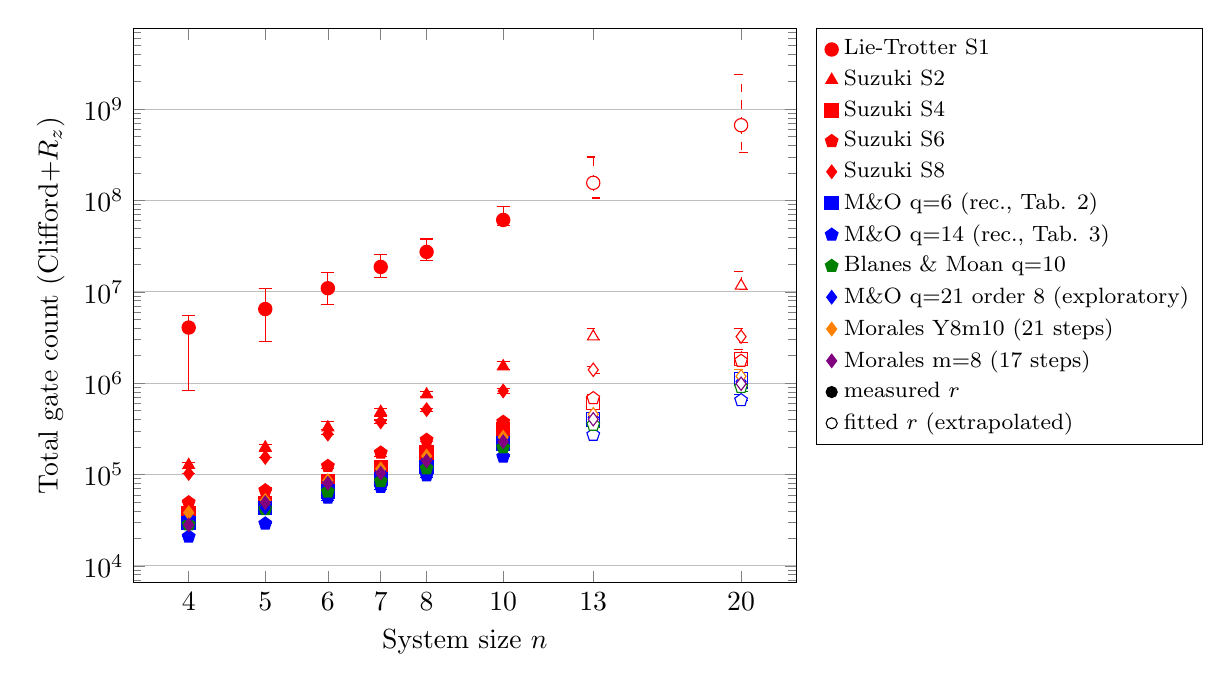
\begin{tikzpicture}
  \begin{loglogaxis}[
    width=10cm,
    xlabel={System size $n$},
    ylabel={Total gate count (Clifford+$R_z$)},
    xtick={4,5,6,7,8,10,13,20},
    xticklabels={4,5,6,7,8,10,13,20},
    ymajorgrids=true,
    legend pos=outer north east,
    legend cell align=left,
    legend style={font=\footnotesize},
  ]
    \addplot[only marks, red, mark=*, mark size=2.4pt, mark options={solid, fill=red}, error bars/.cd, y dir=both, y explicit, error bar style={red}] coordinates {
      (4,4062136) += (0,1411488) -= (0,3228472)
      (5,6480825) += (0,4436575) -= (0,3600025)
      (6,10941840) += (0,5296356) -= (0,3753360)
      (7,18715424) += (0,6624072) -= (0,4347798)
      (8,27344304) += (0,10570768) -= (0,5317104)
      (10,61189570) += (0,24481210) -= (0,7465250)
    };
    \addlegendentry{Lie-Trotter S1}
    \addplot[only marks, red, mark=*, mark size=2.4pt, mark options={solid, fill=white}, forget plot, error bars/.cd, y dir=both, y explicit, error bar style={red, dashed}] coordinates {
      (13,155918893) += (0,143251667) -= (0,49372505)
      (20,666237780) += (0,1729653900) -= (0,329848220)
    };
    \addplot[only marks, red, mark=triangle*, mark size=2.4pt, mark options={solid, fill=red}, error bars/.cd, y dir=both, y explicit, error bar style={red}] coordinates {
      (4,127008) += (0,7200) -= (0,11040)
      (5,197760) += (0,13200) -= (0,20400)
      (6,327600) += (0,49104) -= (0,15120)
      (7,483672) += (0,45864) -= (0,52584)
      (8,750912) += (0,64320) -= (0,40128)
      (10,1524720) += (0,208080) -= (0,126960)
    };
    \addlegendentry{Suzuki S2}
    \addplot[only marks, red, mark=triangle*, mark size=2.4pt, mark options={solid, fill=white}, forget plot, error bars/.cd, y dir=both, y explicit, error bar style={red, dashed}] coordinates {
      (13,3234192) += (0,718224) -= (0,222768)
      (20,11655360) += (0,5156160) -= (0,1104000)
    };
    \addplot[only marks, red, mark=square*, mark size=2.4pt, mark options={solid, fill=red}, error bars/.cd, y dir=both, y explicit, error bar style={red}] coordinates {
      (4,37312) += (0,848) -= (0,0)
      (5,48760) += (0,2120) -= (0,1060)
      (6,83952) += (0,6360) -= (0,3816)
      (7,120946) += (0,11130) -= (0,6678)
      (8,174688) += (0,6784) -= (0,6784)
      (10,310580) += (0,28620) -= (0,7420)
    };
    \addlegendentry{Suzuki S4}
    \addplot[only marks, red, mark=square*, mark size=2.4pt, mark options={solid, fill=white}, forget plot, error bars/.cd, y dir=both, y explicit, error bar style={red, dashed}] coordinates {
      (13,610454) += (0,86814) -= (0,39962)
      (20,1835920) += (0,517280) -= (0,212000)
    };
    \addplot[only marks, red, mark=pentagon*, mark size=2.4pt, mark options={solid, fill=red}, error bars/.cd, y dir=both, y explicit, error bar style={red}] coordinates {
      (4,49536) += (0,0) -= (0,0)
      (5,67080) += (0,5160) -= (0,0)
      (6,123840) += (0,6192) -= (0,6192)
      (7,173376) += (0,7224) -= (0,14448)
      (8,239424) += (0,8256) -= (0,8256)
      (10,376680) += (0,25800) -= (0,15480)
    };
    \addlegendentry{Suzuki S6}
    \addplot[only marks, red, mark=pentagon*, mark size=2.4pt, mark options={solid, fill=white}, forget plot, error bars/.cd, y dir=both, y explicit, error bar style={red, dashed}] coordinates {
      (13,684216) += (0,67080) -= (0,40248)
      (20,1754400) += (0,350880) -= (0,185760)
    };
    \addplot[only marks, red, mark=diamond*, mark size=2.4pt, mark options={solid, fill=red}, error bars/.cd, y dir=both, y explicit, error bar style={red}] coordinates {
      (4,102640) += (0,0) -= (0,0)
      (5,153960) += (0,0) -= (0,0)
      (6,277128) += (0,30792) -= (0,0)
      (7,377202) += (0,17962) -= (0,17962)
      (8,513200) += (0,20528) -= (0,20528)
      (10,821120) += (0,51320) -= (0,51320)
    };
    \addlegendentry{Suzuki S8}
    \addplot[only marks, red, mark=diamond*, mark size=2.4pt, mark options={solid, fill=white}, forget plot, error bars/.cd, y dir=both, y explicit, error bar style={red, dashed}] coordinates {
      (13,1401036) += (0,133432) -= (0,133432)
      (20,3233160) += (0,769800) -= (0,461880)
    };
    \addplot[only marks, blue, mark=square*, mark size=2.4pt, mark options={solid, fill=blue}, error bars/.cd, y dir=both, y explicit, error bar style={blue}] coordinates {
      (4,29348) += (0,1012) -= (0,4048)
      (5,43010) += (0,1265) -= (0,5060)
      (6,65274) += (0,1518) -= (0,3036)
      (7,89436) += (0,4428) -= (0,6198)
      (8,121440) += (0,12144) -= (0,6072)
      (10,218845) += (0,8855) -= (0,13915)
    };
    \addlegendentry{M\&O q=6 (rec., Tab. 2)}
    \addplot[only marks, blue, mark=square*, mark size=2.4pt, mark options={solid, fill=white}, forget plot, error bars/.cd, y dir=both, y explicit, error bar style={blue, dashed}] coordinates {
      (13,399614) += (0,27956) -= (0,8222)
      (20,1110670) += (0,108790) -= (0,43010)
    };
    \addplot[only marks, blue, mark=pentagon*, mark size=2.4pt, mark options={solid, fill=blue}, error bars/.cd, y dir=both, y explicit, error bar style={blue}] coordinates {
      (4,20916) += (0,0) -= (0,0)
      (5,29050) += (0,0) -= (0,0)
      (6,55776) += (0,0) -= (0,3486)
      (7,73206) += (0,0) -= (0,4067)
      (8,97608) += (0,4648) -= (0,4648)
      (10,156870) += (0,5810) -= (0,0)
    };
    \addlegendentry{M\&O q=14 (rec., Tab. 3)}
    \addplot[only marks, blue, mark=pentagon*, mark size=2.4pt, mark options={solid, fill=white}, forget plot, error bars/.cd, y dir=both, y explicit, error bar style={blue, dashed}] coordinates {
      (13,271908) += (0,15106) -= (0,0)
      (20,650720) += (0,92960) -= (0,11620)
    };
    \addplot[only marks, green!50!black, mark=pentagon*, mark size=2.4pt, mark options={solid, fill=green!50!black}, error bars/.cd, y dir=both, y explicit, error bar style={green!50!black}] coordinates {
      (4,28356) += (0,1668) -= (0,0)
      (5,41700) += (0,0) -= (0,2085)
      (6,65052) += (0,0) -= (0,2502)
      (7,84651) += (0,2919) -= (0,2919)
      (8,116760) += (0,6672) -= (0,6672)
      (10,198075) += (0,2085) -= (0,6255)
    };
    \addlegendentry{Blanes \& Moan q=10}
    \addplot[only marks, green!50!black, mark=pentagon*, mark size=2.4pt, mark options={solid, fill=white}, forget plot, error bars/.cd, y dir=both, y explicit, error bar style={green!50!black, dashed}] coordinates {
      (13,349654) += (0,13552) -= (0,18974)
      (20,909060) += (0,75060) -= (0,91740)
    };
    \addplot[only marks, blue, mark=diamond*, mark size=2.4pt, mark options={solid, fill=blue}, error bars/.cd, y dir=both, y explicit, error bar style={blue}] coordinates {
      (4,34720) += (0,0) -= (0,0)
      (5,43400) += (0,4340) -= (0,0)
      (6,83328) += (0,5208) -= (0,5208)
      (7,109368) += (0,6076) -= (0,6076)
      (8,145824) += (0,6944) -= (0,6944)
      (10,243040) += (0,17360) -= (0,8680)
    };
    \addlegendentry{M\&O q=21 order 8 (exploratory)}
    \addplot[only marks, blue, mark=diamond*, mark size=2.4pt, mark options={solid, fill=white}, forget plot, error bars/.cd, y dir=both, y explicit, error bar style={blue, dashed}] coordinates {
      (13,423150) += (0,50778) -= (0,39494)
      (20,1041600) += (0,225680) -= (0,156240)
    };
    \addplot[only marks, orange, mark=diamond*, mark size=2.4pt, mark options={solid, fill=orange}, error bars/.cd, y dir=both, y explicit, error bar style={orange}] coordinates {
      (4,38192) += (0,0) -= (0,0)
      (5,52080) += (0,0) -= (0,0)
      (6,85932) += (0,2604) -= (0,2604)
      (7,115444) += (0,6076) -= (0,0)
      (8,159712) += (0,6944) -= (0,6944)
      (10,256060) += (0,21700) -= (0,4340)
    };
    \addlegendentry{Morales Y8m10 (21 steps)}
    \addplot[only marks, orange, mark=diamond*, mark size=2.4pt, mark options={solid, fill=white}, forget plot, error bars/.cd, y dir=both, y explicit, error bar style={orange, dashed}] coordinates {
      (13,457002) += (0,62062) -= (0,28210)
      (20,1189160) += (0,234360) -= (0,164920)
    };
    \addplot[only marks, violet, mark=diamond*, mark size=2.4pt, mark options={solid, fill=violet}, error bars/.cd, y dir=both, y explicit, error bar style={violet}] coordinates {
      (4,28160) += (0,0) -= (0,0)
      (5,49280) += (0,0) -= (0,0)
      (6,80256) += (0,0) -= (0,4224)
      (7,103488) += (0,4928) -= (0,0)
      (8,140800) += (0,11264) -= (0,0)
      (10,228800) += (0,10560) -= (0,3520)
    };
    \addlegendentry{Morales m=8 (17 steps)}
    \addplot[only marks, violet, mark=diamond*, mark size=2.4pt, mark options={solid, fill=white}, forget plot, error bars/.cd, y dir=both, y explicit, error bar style={violet, dashed}] coordinates {
      (13,402688) += (0,27456) -= (0,18304)
      (20,985600) += (0,154880) -= (0,56320)
    };
    \addlegendimage{only marks, black, mark=*}
    \addlegendentry{measured $r$}
    \addlegendimage{only marks, black, mark=*, mark options={fill=white}}
    \addlegendentry{fitted $r$ (extrapolated)}
  \end{loglogaxis}
\end{tikzpicture}
